%%%%%%%%%%%%%%%%%%%%%%%%%%%%%%%%%%%%%%%%%
% a0poster Landscape Poster
% LaTeX Template
% Version 1.0 (22/06/13)
%
% The a0poster class was created by:
% Gerlinde Kettl and Matthias Weiser (tex@kettl.de)
% 
% This template has been downloaded from:
% http://www.LaTeXTemplates.com
%
% License:
% CC BY-NC-SA 3.0 (http://creativecommons.org/licenses/by-nc-sa/3.0/)
%
%%%%%%%%%%%%%%%%%%%%%%%%%%%%%%%%%%%%%%%%%

%----------------------------------------------------------------------------------------
%	PACKAGES AND OTHER DOCUMENT CONFIGURATIONS
%----------------------------------------------------------------------------------------

\documentclass[a3,portrait,14pt]{sciposter}



\usepackage{multicol,caption} % This is so we can have multiple columns of text side-by-side
\columnsep=20pt % This is the amount of white space between the columns in the poster
\columnseprule=3pt % This is the thickness of the black line between the columns in the poster

\usepackage[svgnames]{xcolor} % Specify colors by their 'svgnames', for a full list of all colors available see here: http://www.latextemplates.com/svgnames-colors

%\usepackage{times} % Use the times font
%\usepackage{palatino} % Uncomment to use the Palatino font

\usepackage{graphicx} % Required for including images
\graphicspath{{figures/}} % Location of the graphics files
\usepackage{booktabs} % Top and bottom rules for table
\usepackage[font=small,labelfont=bf]{caption} % Required for specifying captions to tables and figures
\usepackage{amsfonts, amsmath, amsthm, amssymb} % For math fonts, symbols and environments
%\usepackage{wrapfig} % Allows wrapping text around tables and figures


\usepackage{listings}
\usepackage{amsfonts}
\usepackage{tabularx}
\usepackage{enumitem}

\usepackage{tikz}
\usepackage{graphicx}
\usepackage{subfig}


\usepackage{lipsum}

%\usepackage[boxruled]{algorithm2e}
%\usepackage{algorithm}% http://ctan.org/pkg/algorithm
\usepackage[noend]{algpseudocode}% http://ctan.org/pkg/algorithmicx
\newtheorem{Def}{Definition}
\newtheorem{Theorem}{Theorem}

\usetikzlibrary{arrows,positioning} 


\usetikzlibrary{arrows,positioning} 
\pgfarrowsdeclarecombine{ring}{ring}{}{}{o}{o}

\DeclareMathOperator{\ringarrow}{\raisebox{0.5ex}{\tikz[baseline]{\draw[ring->](0,0)--(2em,0);}}}

\tikzset{
    %Define standard arrow tip
    >=stealth',
    %Define style for boxes
    observed/.style={
           rectangle,
           rounded corners,
           draw=black, thick,
           minimum width=2.5em,
           minimum height=1.5em,
           font=\footnotesize,
           text centered,
           scale=1,
           fill=blue!20!white},
     latent/.style={
           rectangle,
           rounded corners,
           draw=black, thick, dashed,
           minimum width=2.5em,
           minimum height=1.5em,
           font=\footnotesize,
           text centered,
           fill=black!10!white
           },
     empty/.style={
           circle,
           rounded corners,
           minimum width=.5em,
           minimum height=.5em,
           font=\footnotesize,
           text centered,
           },
    % Define arrow style
    pil/.style={
           o->,
           thick,
           shorten <=2pt,
           shorten >=2pt,},
    sh/.style={ shade, shading=axis, left color=red, right color=green,
    shading angle=45 }  
}


\begin{document}
\def\ci{\perp\!\!\!\perp}
%----------------------------------------------------------------------------------------
%	POSTER HEADER 
%----------------------------------------------------------------------------------------

% The header is divided into three boxes:
% The first is 55% wide and houses the title, subtitle, names and university/organization
% The second is 25% wide and houses contact information
% The third is 19% wide and houses a logo for your university/organization or a photo of you
% The widths of these boxes can be easily edited to accommodate your content as you see fit
\begin{minipage}[t]{0.15\linewidth}%
\centering

\includegraphics[height=3cm]{data61} % Logo or a photo of you, adjust its dimensions here
\end{minipage}
\begin{minipage}[b]{0.65\linewidth}
\centering
\resizebox{\linewidth}{!}{\veryHuge \color{NavyBlue} \textbf{Transparancy, Causality \& Fairness}}
 \color{Black}\\ 

\textbf{Finnian Lattimore}\\ % Author(s)
Australian National University\\ % University/organization
finnlattimore@gmail.com

\end{minipage}
\begin{minipage}[t]{0.15\linewidth}
\centering

\includegraphics[height=3cm]{anu-logo-notext}
\end{minipage}


%----------------------------------------------------------------------------------------

\begin{multicols}{2} % This is how many columns your poster will be broken into, a poster with many figures may benefit from less columns whereas a text-heavy poster benefits from more


%----------------------------------------------------------------------------------------
%	INTRODUCTION
%----------------------------------------------------------------------------------------

%\color{DarkSlateGray} % DarkSlateGray color for the rest of the content

\section*{Introduction}

long vs short regressions

The rise of machine learning and big data is accompanied by increasing concerns over transparency and fairness \cite{Barocas2014}. A recent EU directive requires automated decision systems used to profile individuals must provide \textit{"meaningful information about the logic involved."}  and \textit{"shall not be based on special categories of personal data"} \cite{Goodman2016}

\section*{Fairness \& Discrimination}
Consider a binary outcome of interest $Y$, protected variable $X$, other covariates $Z$ and a model $f$ that outputs the probability of a positive $Y$ for each individual.    
\begin{enumerate}
\item \textit{disparate treatment} Two people with otherwise identical attributes should be treated the same. $f(x,z) = f(x',z) \; \forall \; x,x',z$. 
\item \textit{disparate impact} The distribution of the outcome should be the same for all values of the protected variable. $\sum_z f(x,z)P(z|x) = C \; \forall \; x$
\end{enumerate}

\textit{Disparate treatment} can be trivially avoided by excluding the protected variable from the model. However, this is deeply unsatisfying given the presence of proxy variables and can increase bias (figure \ref{fig:recidivism})

Avoiding \textit{disparate impact} may be be expensive in terms of predictive accuracy and/or require \textit{disparate treatment}. 

\begin{figure}[H]
\caption{Proxies}
\label{fig:recidivism}
	\centering    
          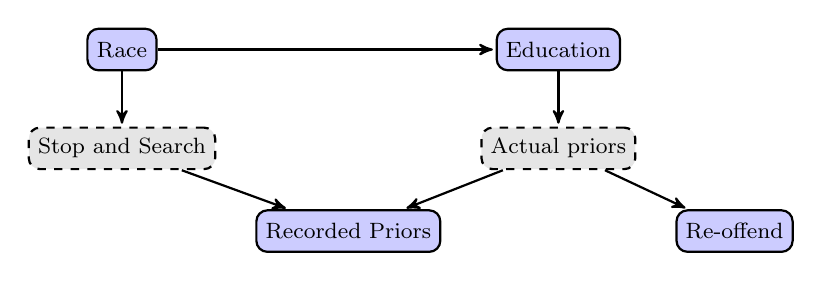
\begin{tikzpicture}[->,>=stealth',shorten >=1pt,auto,node distance=.7cm,
  thick,main node/.style={observed}, hidden/.style={empty},background rectangle/.style={fill=olive!45}]
 %nodes
\node[latent](1){Actual priors};
\node[main node, below left=of 1](2){Recorded Priors};
\node[main node, below right=of 1](3){Re-offend};
\node[latent, above left=of 2](4){Stop and Search};
\node[main node, above=of 4](5){Race};
\node[main node, above=of 1](6){Education};
 \path[every node/.style={font=\tiny}]
    (1) edge (2) edge (3)
    (4) edge (2)
    (5) edge (4) edge (6)
    (6) edge (1);
\end{tikzpicture}
\end{figure}

\section*{Transparancy/Interpretability}
A desire for interpretability implies a miss-match between the real world goal and the optimisation problem presented to a machine learning algorithm \cite{Lipton2016}.
\begin{enumerate}
\item situations where the true objective is hard to measure or quantify. (model can be assessed in multiple different ways for hard to define characteristics such as \textit{fairness}) 
\item integration with human decision making
\item improved generalizability (users can detect and eliminate features that are irrelevant/artefacts of training data)
\item increased \textit{trust} due to the ability to validate the model for problems such as data leaks \& feedback, where acting on model predictions changes the system. 
\item user \textit{trust} leading to increased adherence to the model (irrespective of any actual advantages). 
\end{enumerate}


\section*{Causal Models}
We define a causal model as a model which can be used to predict the outcome of an intervention or change to a system. 

\begin{enumerate}
\item Causal models explicitly predict the outcome of an intervention. If taking actions based on the outcome of the model significantly changes the system, a causal model is required.
\item Interpretable models can mitigate some, but not all problems associated with not building a causal model eg \cite{Caruana2015} (figure \ref{fig:pneumonia}).
\item If a model is non-causal making it transparent can lead to changes in people's behaviour that reduce the predictive accuracy of the model: Consider making the details of an automated essay marking system public. 
\item If membership of a protected class, $X$, is not causally related to the outcome of interest, $Y$, then there exits a set of variables, $Z$, such that $X \ci Y |Z$. 

\end{enumerate}

\begin{figure}[H]
	\caption{Predicting risk of death in pneumonia patients}
	\label{fig:pneumonia}
	\centering    
          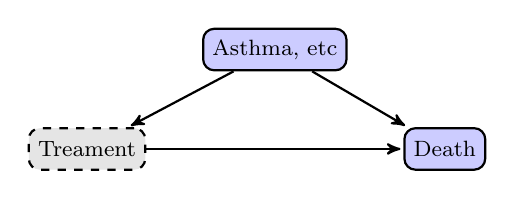
\begin{tikzpicture}[->,>=stealth',shorten >=1pt,auto,node distance=1cm,
  thick,main node/.style={observed}, hidden/.style={empty},background rectangle/.style={fill=olive!45}]
 %nodes
\node[main node](1){Asthma, etc};
\node[latent, below left=of 1](2){Treament};
\node[main node, below right=of 1](3){Death};
 \path[every node/.style={font=\tiny}]
    (1) edge (2) edge (3)
    (2) edge (3);
\end{tikzpicture}
\end{figure}

%\section*{Questions}
%\begin{itemize}
%\item Does causality play a role in the definition of discrimination?
%\item Under what assumptions do causal models generalize better?
%\end{itemize}

%----------------------------------------------------------------------------------------
%	CONCLUSIONS
%----------------------------------------------------------------------------------------

\color{SaddleBrown} % SaddleBrown color for the conclusions to make them stand out

\color{DarkSlateGray} % Set the color back to DarkSlateGray for the rest of the content

 %----------------------------------------------------------------------------------------
%	REFERENCES
%----------------------------------------------------------------------------------------

\bibliographystyle{plain} % Plain referencing style
\bibliography{/home/finn/phd/Causality-Interpretability_and_Ethics} % Use the example bibliography file sample.bib


\end{multicols}
\end{document}
